% !TEX root = EUDAQUserManual.tex
\section{Introduction}
The EUDAQ software is a data acquisition framework, written in C++,
and designed to be modular and portable, running on Linux, Mac OS X, and Windows.
It was originally written primarily to run the EUDET-type beam telescope~\cite{Roloff:2009zza,Jansen:2016},
but is designed to be generally useful for other systems.

The hardware-specific parts are kept separate from the core,
so that the core library can still be used independently.
For example, hardware-specific parts are two components for the EUDET-type beam telescope: \gls{TLU} and \gls{NI} system for Mimosa 26 sensor read out.

The raw data files generated by the DAQ can be converted to the \gls{LCIO} format,
allowing analysis of the data using the EUTelescope package \cite{eutel2008}.

\subsection{Architecture}
It is split into a number of different processes,
each communicating using TCP/IP sockets (see \autoref{fig:DAQ}).
A central Run Control provides an interface for controlling the whole DAQ system;
other processes connect to the Run Control to receive commands and to report their status.

\begin{figure}[htb]
  \begin{center}
    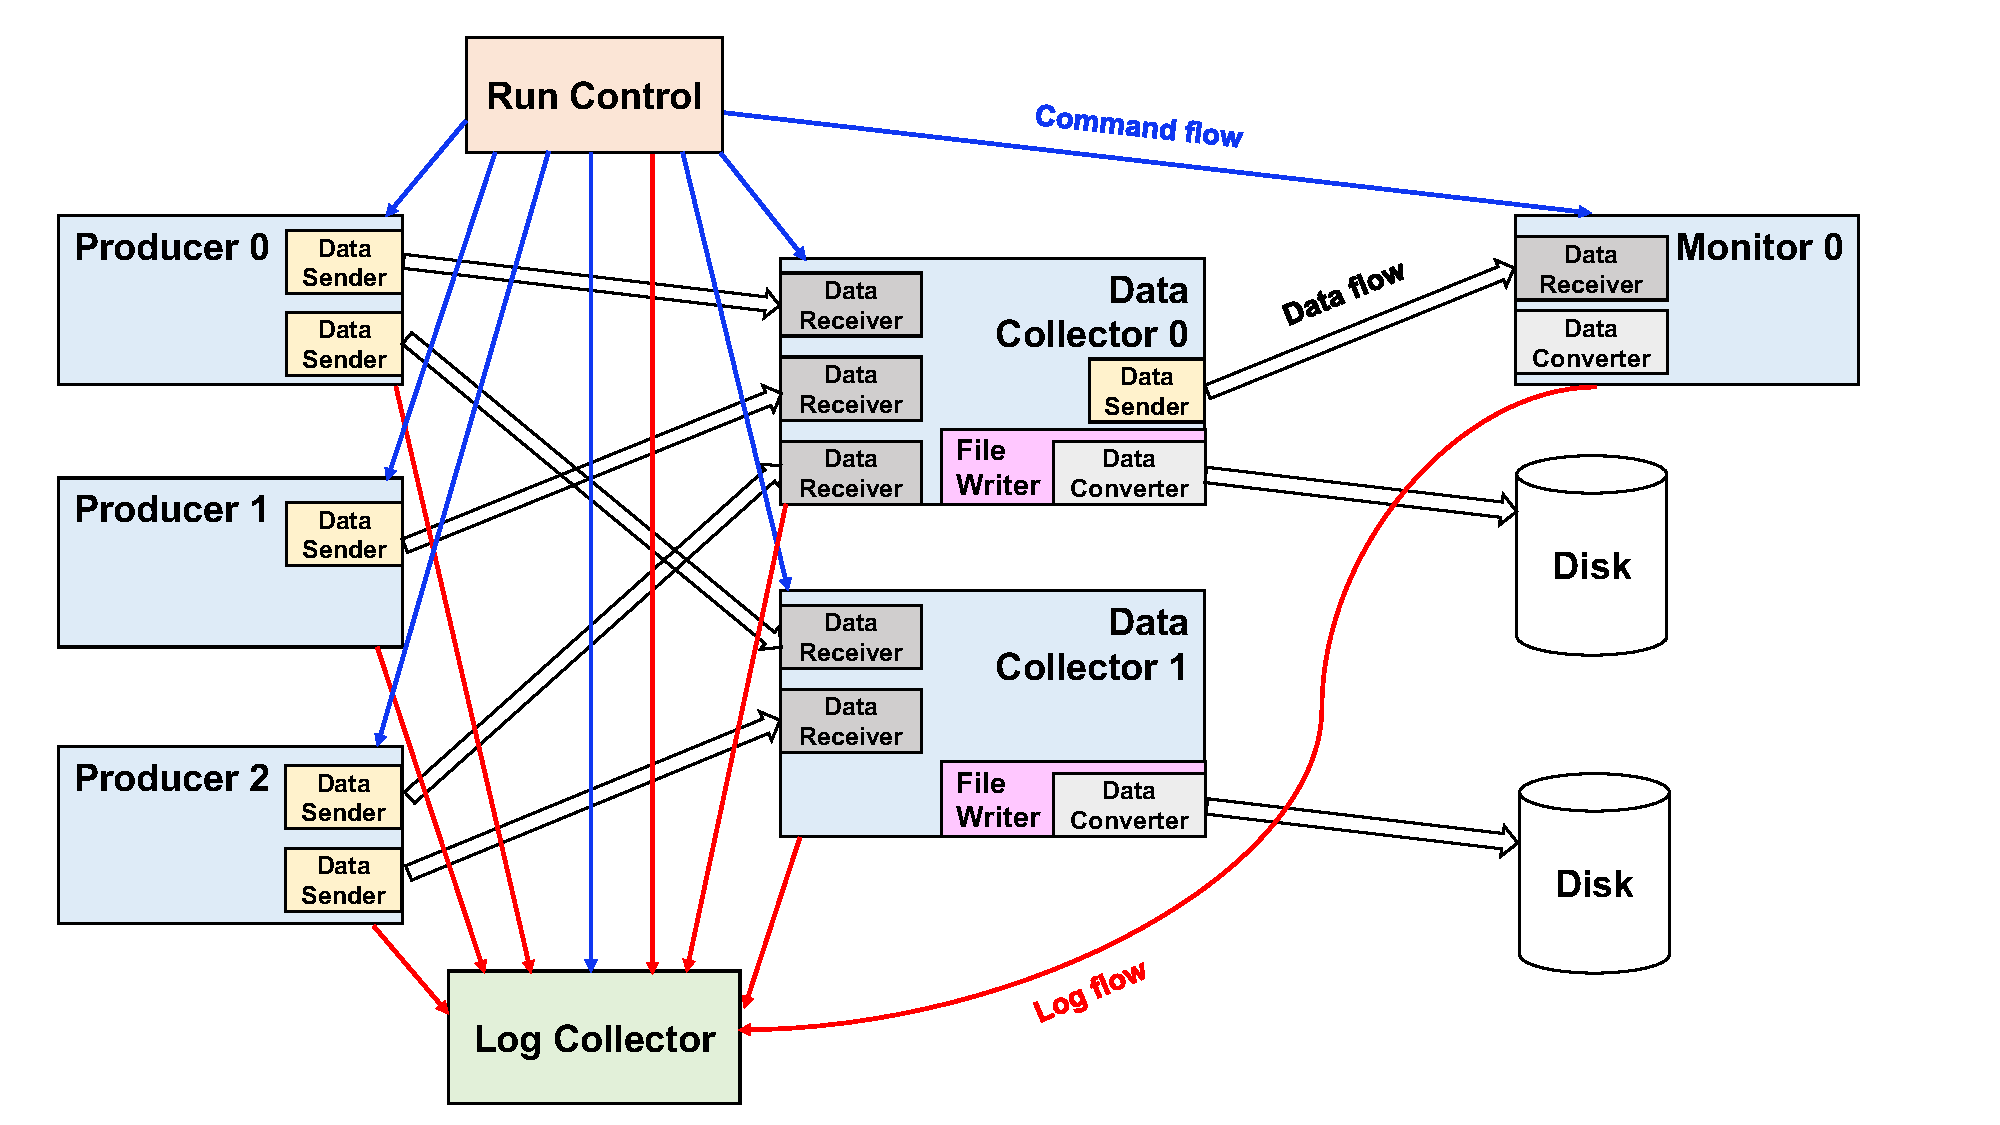
\includegraphics[width=0.9\textwidth]{src/images/eudaq_working_principle}
    \caption{Schematic of the EUDAQ architecture \cite{Spannagel:2016}.}
    \label{fig:DAQ}
  \end{center}
\end{figure}


The DAQ system is made up of a number of different processes that may all be run on the same,
or on different computers. 

\subsubsection{Run Control}
The RunControl is the controller process which manages the full EUDAQ system. There should be always only one instance of RunControl for a runtime setup. All other data taking processes must have the network location of RunControl and anounces themelves to the RunControl. The RunControl takes in the paths of ini/config files and picks up and sends the correlated section to each of the connected processes. As the front end point to users, the RunControl will wait for user input by command line or GUI button click and issue the data taking command to whole EUDAQ system.

\subsubsection{Producer}
Each hardware that produces data will have a Producer process (on the left in \autoref{fig:DAQ}).
This will initialize, configure, stop and start the hardware by receiving the commands from the Run Control (red arrows), read out the data and send it to the Data Collector (blue arrows).

\subsubsection{Data Collector}
The Data Collector is the process that collects all the raw data from the Producers,
merges all the connected incoming streams into a single data stream, and writes it to file.\\

The Data Collector receives all the data streams from all the Producers,
and combines them into a single stream that is written to disk (Storage).
It writes the data in a native raw binary format,
but it can be configured to write in other formats, such as \gls{LCIO}.

\subsubsection{Log Collector}
The Log Collector receives log messages from all other processes (grey arrows),
and displays them to the user, as well as writing them all to file.
This allows for easier debugging, since all log messages are stored together in a central location.

\subsubsection{Monitor}
The Monitor reads the data file and generates online-monitoring plots for display.
In the schematic it is shown to communicate with the Data Collector via a socket,
but it actually just reads the data file from disk.\\

The Online Monitor can be run in one of two modes: online or offline.
In online mode, it connects to the Run Control, so it will know when new runs are started,
and it will automatically open each new data file as it is created.



\subsection{Directory and File Structure}
The EUDAQ software is split into several parts that can each be compiled independently,
and are kept in separate subdirectories.
The general structure is outlined below:

\begin{myitemize}
\item \texttt{main}
  contains the core EUDAQ library with the parts that are common to most of the software,
  and several command-line programs that depend only on this library.
  All definitions in the library should be inside the \texttt{eudaq} namespace.
  It is organized into the following subdirectories:
  \begin{myitemize}
  \item \texttt{main/lib/core}
    contains the source code of the core library,
  \item \texttt{main/lib/lcio}
    contains the source code of the LCIO extension library,
  \item \texttt{main/lib/root}
    contains the source code of the ROOT extension library,
  \item \texttt{main/module}
    contains the source code of the module libraries,
  \item \texttt{main/exe}
    contains the CLI (command line interface) executables source code,
  \end{myitemize}
\item \texttt{gui}
  contains the graphical programs that are built with Qt, such as the RunControl and LogCollector.
\item \texttt{user}
  contains all user provided code shipped with the EUDAQ
  distribution, for example:
  \begin{myitemize}
\item \texttt{user/example}
  contains example code for the integration of user-provided code.
\item \texttt{user/eudet}
  contains the parts that depend on the EUDET-type telescope.
\item e.g. \texttt{user/calice}, \texttt{user/itkstrip}\ldots{}
  contain the code from third-party users.
  \end{myitemize}
\item \texttt{extern}
  global folder which contains external software which themselves are not part of the EUDAQ project.
\item \texttt{cmake}
  global folder which contains cmake files.
\item \texttt{etc}
  contains configuration files of the EUDAQ installation.
\item \texttt{conf}
  contains configuration files for running the beam telescope.
\item \texttt{doc}
  contains source files of the documentation, such as this manual.
\end{myitemize}

Each directory containing code has its own \texttt{src} and \texttt{include} subdirectories,
as well as a local \texttt{CMakeLists.txt} and an optional \texttt{cmake} folder containing the rules
for building that directory using \texttt{CMake}.
Header files have a \texttt{.hh} extension so that they can be automatically recognized as C++,
and source files have either \texttt{.cc} for parts of libraries and \texttt{.cxx} for executables.
In the case of requiring any external dependencies, there could be a local \texttt{extern} folder.

Each directory can contain a \texttt{README.md} file for brief documentation for this specific part, e.g.  
as an installation advice. 
Using the \texttt{*.md} file ending allows the Markdown language \cite{markdownWWW} to be applied. 
Accordingly, the content will be formatted on the the GitHub platform, where the code is hosted online.

\subsection{Executables}
All executable programs from the different subdirectories are in the \texttt{bin} subdirectory. They should all accept a \texttt{-h} (or \texttt{--help}) command-line parameter, which will provide a summary of possible different command-line options.

The executable programs can be split into two different categories: firstly, processes, which are used for the data acquisition and communicating with the Run Control (DAQ); and, secondly, utilities, which are used before or after the data taking in order to access the data files (Test, Development, Tools).
In \autoref{tab:exesall}, an overview of the most important EUDAQ executables is given.

\begin{table}
\centering
\small
\begin{tabular}{ c | l | l | p{4cm}}
  \textbf{Binary} & \textbf{Category} & \textbf{GUI/CLI}  & \textbf{Description}\\
  \hline
  \hline
  \texttt{euRun} & Run Control & GUI & (Sec. \ref{sec:runcontrol}) \\
  \texttt{euLog} & Log Collector & GUI & (Sec. \ref{sec:logcollector}) \\
  \texttt{StdEventMonitor} & legacy Monitor & GUI & \\
  \texttt{euCliRun} & Run Control & CLI & (Sec. \ref{sec:runcontrol}) \\
  \texttt{euCliLogger} & Log Collector & CLI & (Sec. \ref{sec:logcollector}) \\
  \texttt{euCliCollector} & Data Collector & CLI & (Sec. \ref{sec:datacollector}) \\
  \texttt{euCliProducer} & Producer & CLI & (Sec. \ref{sec:testproducer}) \\
  \texttt{euCliMonitor} & Monitor & CLI & (Sec. \ref{sec:onlinemonitor}) \\
  \hline
  \texttt{euCliConverter} & Offline Tool & CLI & data file converter (Sec. \ref{sec:convertafterdatatacking}) \\
  \texttt{euCliReader} & Offline Tool & CLI & dump events from data file (Sec. \ref{sec:dumpafterdatatacking}) \\
  
\end{tabular}
\caption{Overview of EUDAQ executables.}
\label{tab:exesall}
\end{table}


\subsection{Libraries}
The libraries are installed in the \texttt{lib} directory under the install path in Linux/MacOS systems, and to the \texttt{bin} sub-folder in Windows systems. The suffix of libraries name can be \texttt{.so}, \texttt{.dylib}, \texttt{.dll} depending on operate systems. There are 3 category of libraries: core, extension and module: 

\begin{itemize}
\item Core: the core library. It should be always built and installed.
\item Extension: optional features of EUDAQ (e.g.\ support for external data format). Static linked core library.
\item Module: user module. Dynamic load by EUDAQ core library at run-time.
\end{itemize}

In \autoref{tab:liball}, an overview of the all EUDAQ libraries is given.\\

\begin{table}
\centering
\small
\begin{tabular}{ l | l | l | p{4cm}}
  \textbf{Binary} & \textbf{Category} & \textbf{Source Code} & \textbf{Description}\\
  \hline
  \hline
  \texttt{libeudaq\_core} & Core & main$\backslash$lib$\backslash$core & core library \\
  \hline
  \texttt{libeudaq\_lcio} & Extension & main$\backslash$lib$\backslash$lcio & lcio extension library \\
  \texttt{libeudaq\_std} & Extension & main$\backslash$lib$\backslash$std & standard extension library \\
  \hline
  \texttt{libeudaq\_module\_test} & Module & main$\backslash$module$\backslash$test & test module library \\
  \texttt{libeudaq\_module\_example} & Module & user$\backslash$example$\backslash$module &  module library by example user\\
\end{tabular}
\caption{Overview of EUDAQ libraries.}
\label{tab:liball}
\end{table}
